\documentclass[titlepage, 11pt]{article}
\usepackage[a4paper, total={6in, 9.5in}]{geometry}
\usepackage{graphicx}
\usepackage{amsfonts,amssymb}
\usepackage{amsmath}
\usepackage{listings}
\usepackage{booktabs}
\usepackage[T1]{fontenc}
\usepackage{color}
\usepackage{minted}
\usepackage[colorlinks=true, linkcolor=blue, urlcolor=blue, citecolor=blue, pdfborder={0 0 255}]{hyperref}
\usepackage{colortbl}
\usepackage{url}
\usepackage{xcolor}
\usepackage{caption}
\usepackage{subcaption}
\usepackage{dirtytalk}
\usepackage[semicolon, round]{natbib}
\usepackage[ruled]{algorithm2e}
\captionsetup[table]{skip=10pt}
\renewcommand{\vec}[1]{\mathbf{#1}}
\SetKwComment{Comment}{$\triangleright$\ }{}
 \hypersetup{%
 	colorlinks=true,
 	linkcolor=blue,
 	linkbordercolor={0 0 1}
 }

\renewcommand\lstlistingname{Algorithm}
\renewcommand\lstlistlistingname{Algorithms}
\def\lstlistingautorefname{Alg.}

\lstdefinestyle{Python}{
	language        = Python,
	frame           = lines, 
 	basicstyle      = \footnotesize,
    numbers         = left,
    stepnumber      = 1,
 	keywordstyle    = \color{red},
 	stringstyle     = \color{blue},
 	commentstyle    = \color{orange}\ttfamily
}

 \setlength{\parindent}{0.0in}
 \setlength{\parskip}{0.05in}

\newcommand{\argmin}{\mathop{\mathrm{argmin}}}
\newcommand{\argmax}{\mathop{\mathrm{argmax}}}
\newcommand{\minimize}{\mathop{\mathrm{minimize}}}
\newcommand{\maximize}{\mathop{\mathrm{maximize}}}
\newcommand{\st}{\mathop{\mathrm{subject\,\,to}}}
\newcommand{\dist}{\mathop{\mathrm{dist}}}
\newcommand{\norm}[1]{\left\lVert#1\right\rVert}
\renewcommand{\vec}[1]{\mathbf{#1}}

\def\R{\mathbb{R}}
\def\E{\mathbb{E}}
\def\P{\mathbb{P}}
\def\S{\mathbb{S}}
\def\Cov{\mathrm{Cov}}
\def\Var{\mathrm{Var}}
\def\half{\frac{1}{2}}
\def\quat{\frac{1}{4}}
\def\sign{\mathrm{sign}}
\def\supp{\mathrm{supp}}
\def\th{\mathrm{th}}
\def\tr{\mathrm{tr}}
\def\dim{\mathrm{dim}}
\def\dom{\mathrm{dom}}

\begin{document}
 
\title{
    {EE2703: Function Optimization} \\~\
    {\vlarge Programming Assignment {\#} 6}\
}
\author{Student Name, Roll Number\
: & Annangi Shashank Babu, EE21B021}
\date{\today}     
\maketitle
\setcounter{page}{0}

\newpage

\section{Gradient decent for single variable}
\begin{flushleft}
Imagine you are trying to climb down a hill.

At the top of the hill, you take a step in a random direction. You look around and see which direction will take you closer to the bottom of the hill. Then you take a step in that direction. You repeat this process, taking steps in the direction that takes you closer to the bottom of the hill each time, until you finally reach the bottom.

This is what gradient descent is like. Instead of a hill, we have a graph. At the top of the graph, and we look around to see which direction takes us closer to the minimum value . Then we take a step in that direction, and we keep repeating this process, until we finally reach the minimum value (Not nesseccaryly the global minima).

Gradient descent is a way for a computer to find the minimum value of a function by taking steps in the direction that minimizes the function at each step.
\end{flushleft}
\begin{center}
\begin{algorithm}[]\label{alg1}

\For{$i=0$ to $totalsteps$}{
$minx \gets minx - slope*alpha$\;
}
 \caption{Gradient decent algorithm for single variable}
\end{algorithm}
\end{center}
\lstinputlisting[style=Python]{al.py}
\begin{figure}[ht]
    \centering
    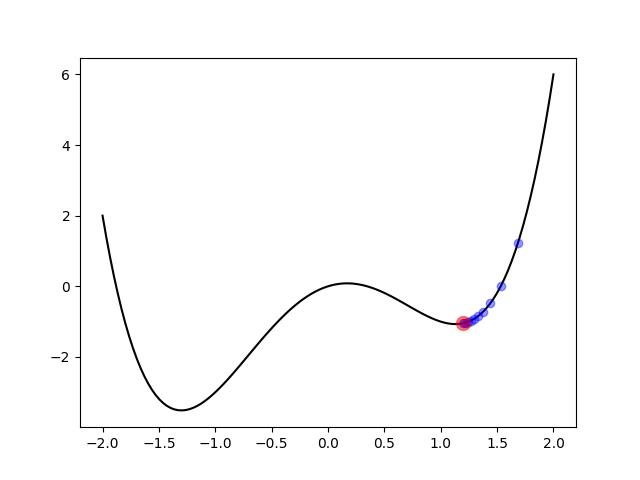
\includegraphics[width=1\textwidth]{gradient_decent_single_variable.jpg}
    \caption{gradient decent for single variable}
    \label{fig:gradient_decent_single_variable-png}
\end{figure}
\section{Gradient decent for two variables}
\begin{flushleft}
    The algorithm is the same as the case of single variable, just that the \textbf{Gradient Vector} evaluated at the current point conveys the direction towards the minimum.
\end{flushleft}
\lstinputlisting[style=Python]{bl.py}
\begin{figure}[ht]
    \centering
    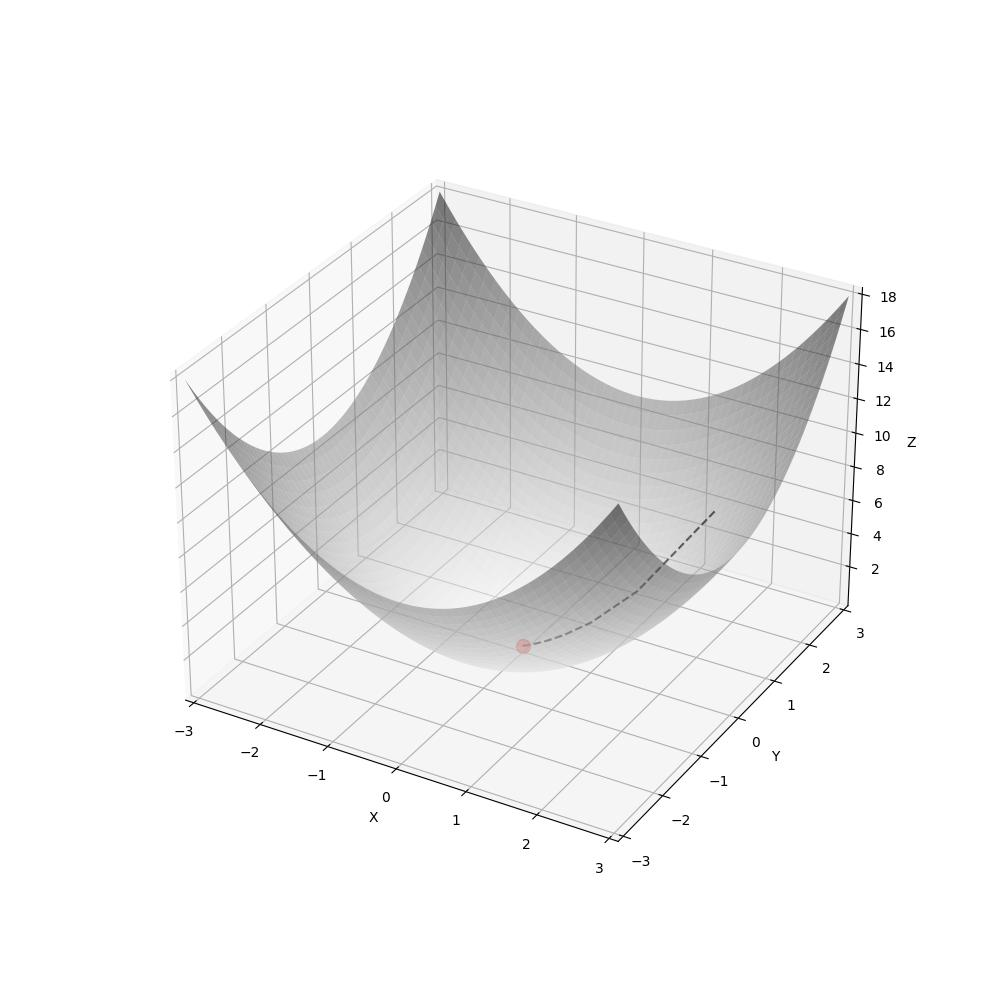
\includegraphics[width=0.8\textwidth]{gradient_decent_two_variable.jpg}
    \caption{Gradient decent in case of 2 variables}
    \label{fig:gradient_decent_singel_variable-png}
\end{figure}
\section{Multi-variable Gradient decent}
\begin{flushleft}
    Extending the above concept for Multivariable funtion, The Gradient decent function is modified as :
\end{flushleft}
\begin{note}[Note]
    The dfunc input to the below function is not nessecary, the partial derivative is calculated from the formula : $(f(x + dx) - f(x))/ dx$
\end{note}
\lstinputlisting[style=Python]{cl.py}
\begin{example}
    The output for the function $w^2 = (x-2)^2 + y^2 + (z-0.5)^2$ is as follows : 
    \\
    \\
    The input vector at close to which minimum occurs is [2.00010986e+00 \: 3.19572276e-04 \: 5.00267143e-01], the minimum value of the function is nearly 
    1.855606530953801e-07
\end{example}
\section{Given Testcases}
\subsection{Single variable}
\subsubsection{testcase 1}
The output for the function \\
\begin{center}
$f(x) = x^2 + 3*x + 8$ 
\end{center}
\begin{figure}[ht]
    \centering
    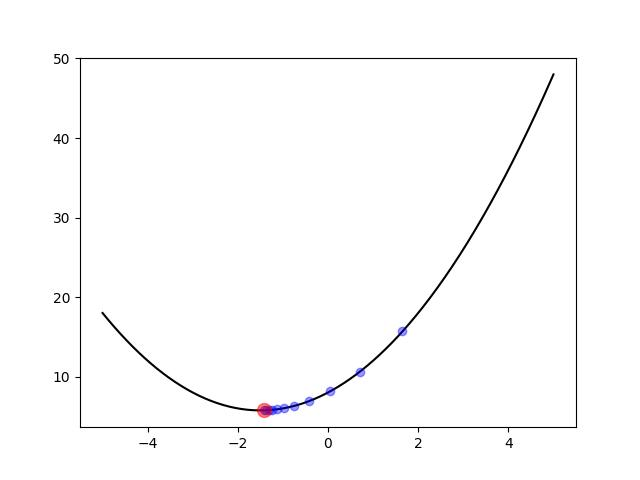
\includegraphics[width=0.8\textwidth]{testcase_single_variable.jpg}
    \caption{Output for single variable testcase}
    \label{fig:testcase single variable jpg}
\end{figure}
The output for the function \\
\begin{center}
$f(x) = cos(x)**4 - sin(x)**3 - 4*sin(x)**2 + cos(x) + 1$
\end{center}
The output to the code is : \\
Min occurs at x = -1.500004999989926,where y = 5.75000000002
50004
\subsubsection{testcase 2}
\begin{figure}[ht]
    \centering
    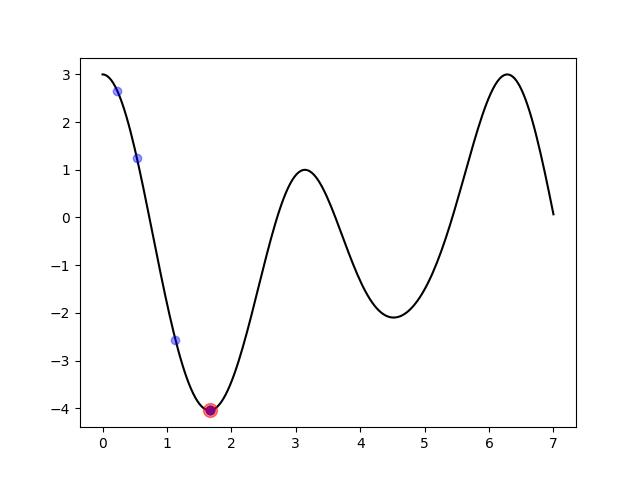
\includegraphics[width=0.8\textwidth]{testcase_single_variable_2.jpg}
    \caption{testcase single variable case 2}
    \label{fig:test casesingle variable 2}
\end{figure}

The output to the code is : \\
Min occurs at x = 1.6616558120457037,where y = -4.0454120514
35421

\subsection{Two Variable}
\subsubsection{testcase 1}
The output for the function \\
\begin{center}
    $f(x,y) = x^4 + 16x^3 + 96x^2 - 256x + y^2 - 4y + 262$
\end{center}
\begin{figure}[ht]
    \centering
    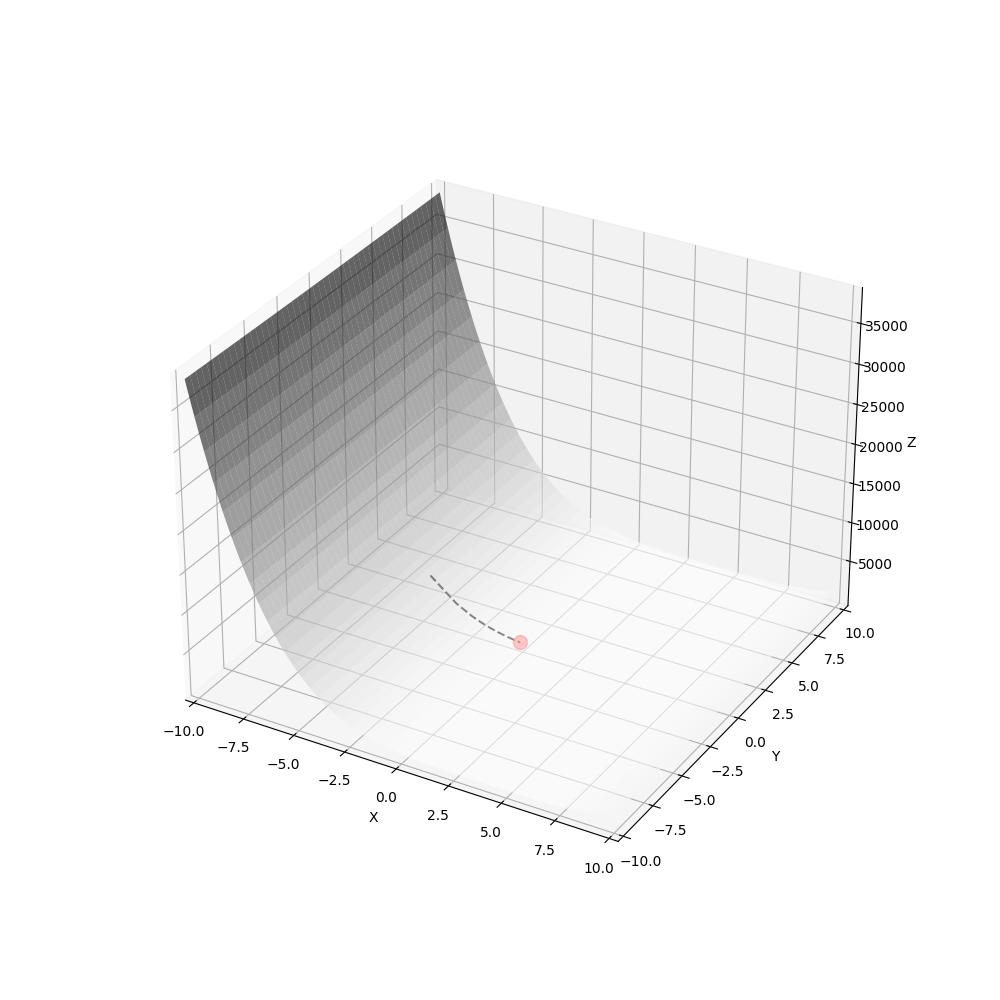
\includegraphics[width=0.8\textwidth]{testcase_gradient_decent_two_variable.jpg}
    \caption{Output for two variable, only for first 10 steps}
    \label{fig:Output for two variable}
\end{figure}
The minima point from the code : 
Min at x = 3.842076451759965, y = 1.9999159987690973,z =
 2.0006220030289796

\subsubsection{testcase 2}

The output for the function \\
\begin{center}
    $f(x,y) = exp(-(x - y)**2)*sin(y)$
\end{center}
\begin{figure}[ht]
    \centering
    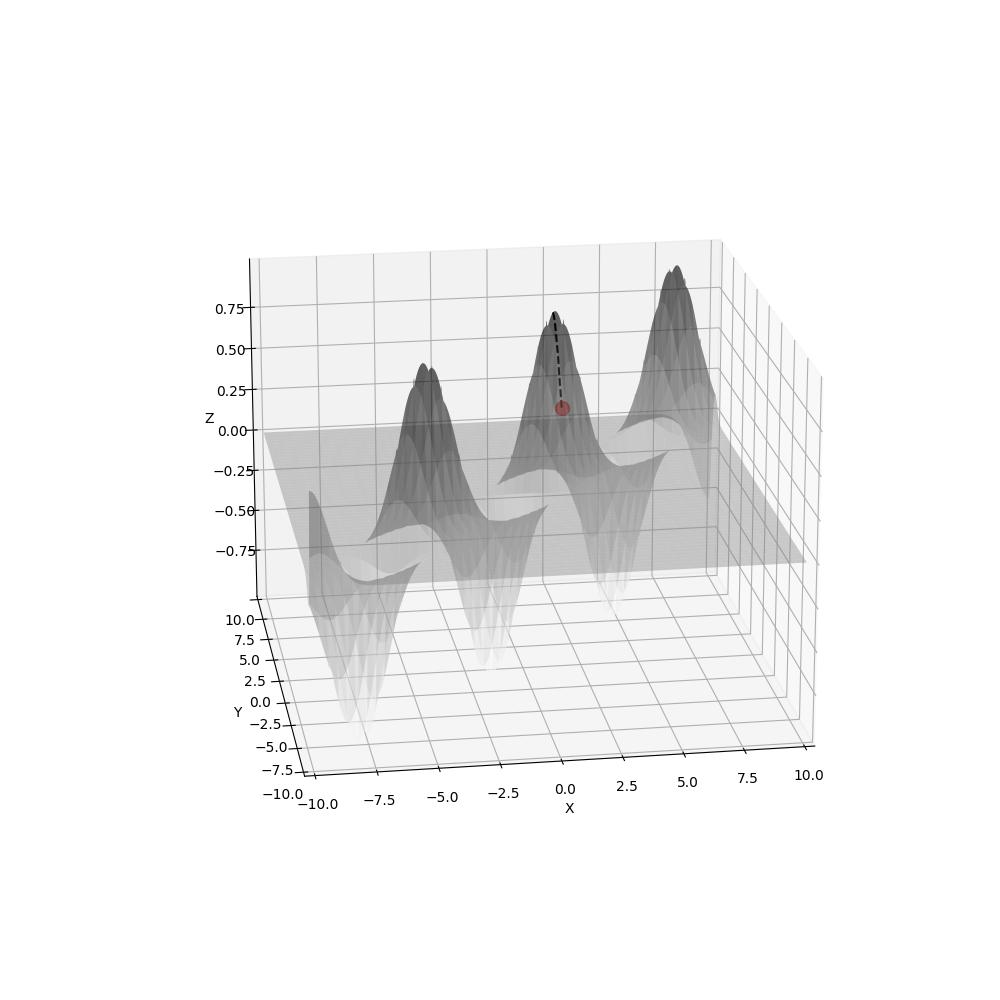
\includegraphics[width=0.8\textwidth]{testcase_gradient_decent_two_variable_case_2.jpg}
    \caption{Output for two variable, only for first 10 steps}
    \label{fig:Output for two variable}
\end{figure}
The minima point from the code : 
Maximum at x = -1.570766326776594, y = -1.5707713267813568,z
 = -0.9999999996624996



%%%%%%%%%%%%%%%%%%%%%%%%%%%%%%%%%

% Uncomment the lines below to add references using bibtex.
% \bibliographystyle{plainnat}
% \bibliography{references}

\end{document}

